We compare the performance of 4 memory management strategies 
\begin{description}
\setlength{\itemsep}{0pt}
  \setlength{\parskip}{0pt}
\item[\none] -- which does no compaction of the data, this was previously the default in HBase.
\item[\basic] -- which compacts the representation of the index; this is the default in HBase 2.0.
\item[\eager] -- which compacts both the data and index.
\item[\magic] -- which compacts the index or both the data and the index based on the workload.
\end{description}

We compare the strategies by measuring their throughput and latency. In addition we measure the write volume, that is the number of KB written to the file system, and the cumulative gc time of each run.

The results of the following experiments are presented:
(1) demonstrating the insight from different sets of experiments showing that gc overhead is a great throughput predictor,
(2) write-only workload - comparing all 4 strategies,
(3) mixed read-write workload - showing reduction in read latencies of \basic\ and \magic\ strategies with respect to \none.
(4) evaluating different settings of the \basic\ strategy in order to find its optimal configuration,

\paragraph{Experiment setup.}

Our experiments run on 2 clusters with different hardware. 
The first cluster consists of five 12-core Intel Xeon 5 machines with 48GB RAM and 3TB 
SSD storage, interconnected by 1G Ethernet. 
The second cluster consists of five 8-core 
Intel Xeon E5620 servers with 24GB RAM and 1TB magnetic drive. The interconnects  are 1Gbps Ethernet. 
We denote these clusters as the SSD cluster and HDD cluster, respectively.
In both clusters we allocate three nodes to HBase nodes, 1 master and 2 region servers, one to simulate the client whose performance we measure, and one to simulate background traffic
as explained below. Each HBase node runs both an HBase region server or master and the underlying 
Hadoop File System (HDFS) server.
 
A region server runs within 8GB JVM container, with G1GC memory management. We use default configuration which allocates 40\% of the heap to memstore (roughly 3GB) and 40\% of the heap to block cache. 
Number of number of flush threads is set to 10, and  the limit on number of store files before blocking is set to 25.

The traffic is driven by a client running the popular YCSB benchmark~\cite{Cooper}. 
We run write-only and mixed read-write workload where keys are chosen from either a zipfian or a uniform distribution over a data set of 100 millions items.
In all the experiments we create a table with 4 columns (in a single column family) which is pre-split into 50 regions. 
Each update operation writes 25 Bytes values to all 4 columns of a single key, namely writing 100 Bytes of data. To increase the load updates are batched at the client side; buffer size is 10KB
Each read operation reads a single column of a single key (a cell).


\paragraph{GC overhead.}

Our experiments show that in write-only workloads gc and throughput have a very high correlation. 
Figure~\ref{fig:gc-throughput-log2} plots the scatter graph of cumulative gc time vs write throughput of several write-only experiments with varying settings in different strategies. It clearly shows that  the lower the gc overhead is, the higher the throughput is.
Specifically, there is a negative linear correlation between their values on a log-log scale.

\begin{figure}[htb]
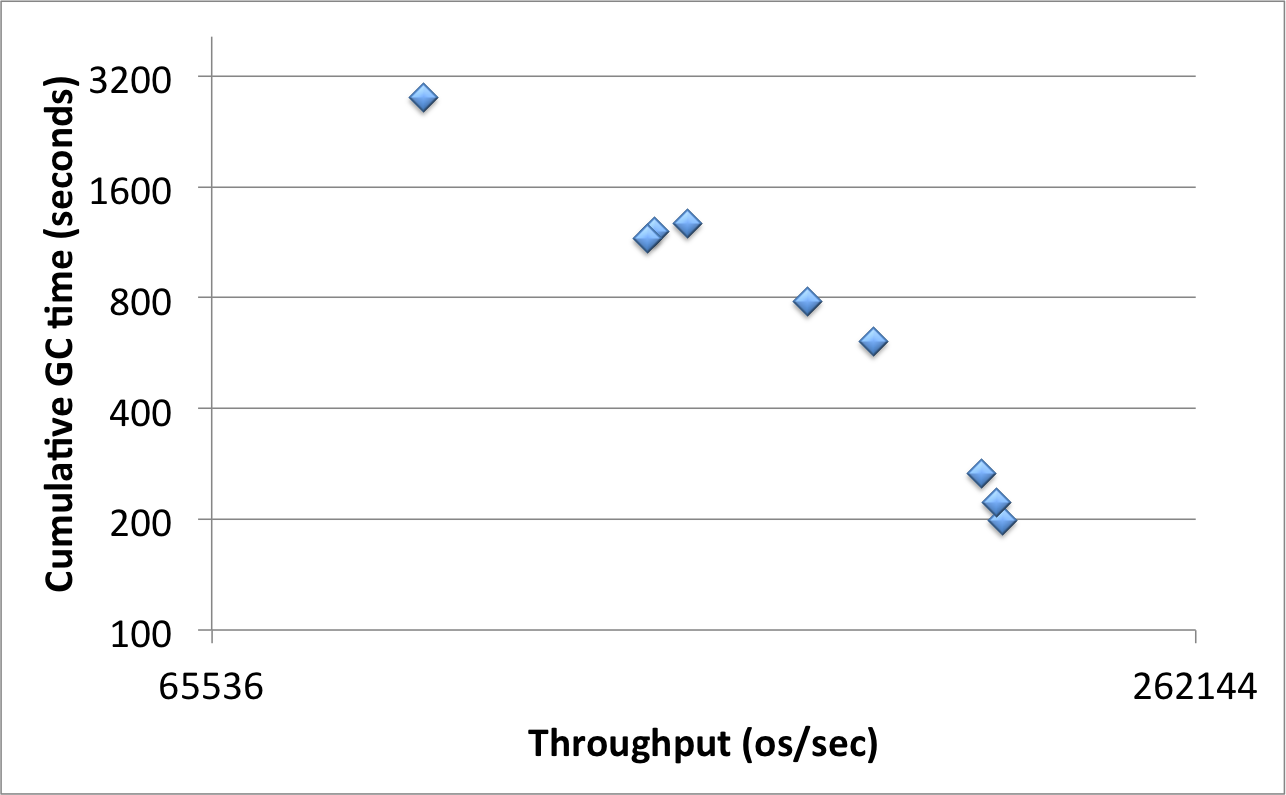
\includegraphics[width=\figw]{Figs/gc-throughput-log2.png}
\caption{{\bf GC-Throughput correlation.} Log-log scale plot of the cumulative gc time vs write throughput in different settings shows negative linear correlation.
}
\label{fig:gc-throughput-log2}
\end{figure}


\paragraph{Write-only workload.}
Each run creates an empty 50 regions table and then utilizes 12 threads to run 500 million update operations, each writing to all columns. Each such run is repeated 5 times. 
We measure total  throughput and total volume of MB written to files. We present here the performance results of the run with the median throughput among 5 runs.

Figures~\ref{fig:throughput-ssd} and~\ref{fig:throughput-hdd} depict the lift in throughput \basic, \magic, and \eager\ achieve over \none in ssd and hdd, respectively.
Tables~\ref{fig:counters:ssd} and ~\ref{fig:counters:hdd} present the number of flushes, disk compactions and WAL files generated during the experiment.
Figures~\ref{fig:volume-ssd} and~\ref{fig:volume-hdd} depict the write volume in every setting. 
\magic demonstrates the tradeoff between throughput and write volume. As we increase the compaction threshold more in-memory compaction are triggered which degrades the throughput but at the same time reduces the write volume.
At the extremes are \basic\ with the highest throughput and \eager with lowest write volume.
\basic\ and \magic\ both run with $2\%$ active segment. In SSD the limit on the size of the pipeline is 5 and in HDD it is 4.
\eager\ runs with $25\%$ active segments and limit of 2 on the size of the pipeline.
The uniques thresholds for \magic\ are $0.2$, $0.35$, and $0.5$.



\begin{figure}[htb]
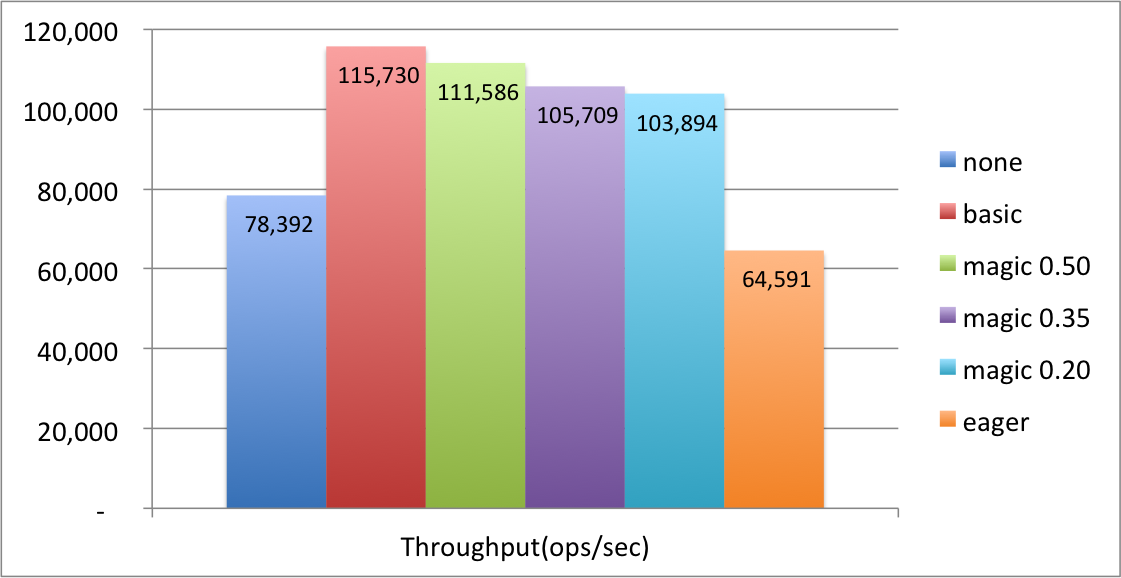
\includegraphics[width=\figw]{Figs/throughput-ssd.png}
\caption{{\bf  Throughput measured in SSD.} Zipfian distribution.
}
\label{fig:throughput-ssd}
\end{figure}

\begin{figure}[htb]
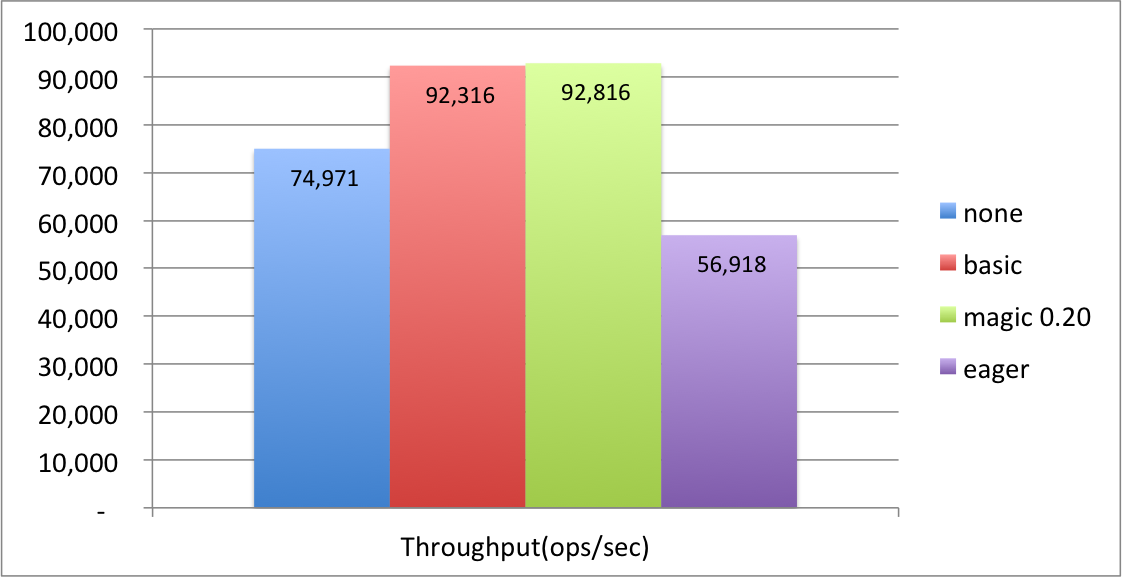
\includegraphics[width=\figw]{Figs/throughput-hdd.png}
\caption{{\bf  Throughput measured in HDD.} Zipfian distribution. 
}
\label{fig:throughput-hdd}
\end{figure}


\begin{figure}[!t]
  \centering
  
  \begin{subfigure}[tb]{\columnwidth}
      \centering\small
    \begin{tabular}{|c|c|c|c|}
      \hline
      Strategy & $\#$flushes & $\#$compactions & $\#$WAL files\\
      %\hline
      \hline
      \none & 1468	&524&	789 \\
\basic & 1224&	355&	806 \\
\magic\ 0.50 &922&	309&	678 \\
\magic\ 0.35 & 754&	261&	615 \\
\magic\ 0.20 & 631	&209	&533 \\
\eager\ & 695	&242&	490 \\
      \hline
    \end{tabular}
	\caption[]{SSD}
    \label{fig:counters:ssd}
  \end{subfigure}
  
  \begin{subfigure}[t]{\columnwidth}
    \centering\small
    \begin{tabular}{|c|c|c|c|c|}
      \hline
        Strategy & $\#$flushes & $\#$compactions & $\#$WAL files\\
      %\hline
      \hline
      \none & 1504 & 548 & 743 \\
\basic & 1210 & 443 & 808 \\
\magic\ 0.50 & 879 & 316 & 695 \\
\magic\ 0.35 & 711 & 248 & 650 \\
\magic\ 0.20 & 630 & 216 & 556 \\
\eager\ & 667 & 242 & 536 \\
      \hline
    \end{tabular}
	\caption[]{HDD}
    \label{fig:counters:hdd}
  \end{subfigure}


  \caption{Number of flushes, disk compactions, and WAL files created in different settings}
  \label{fig:counters}
\end{figure}


\begin{figure}[htb]
%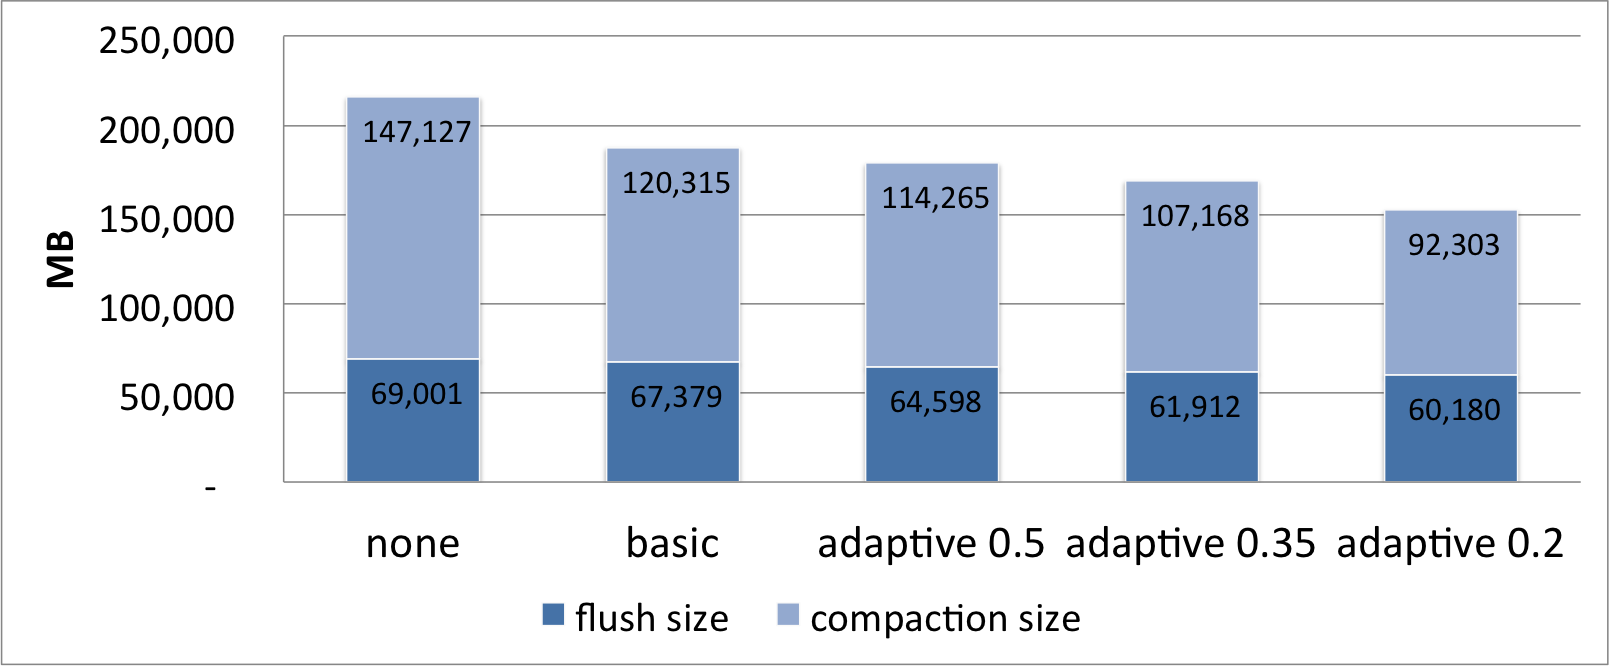
\includegraphics[width=\figw]{Figs/volume-ssd.png}
\caption{{\bf  Write volume in SSD.} Zipfian distribution.
}
\label{fig:volume-ssd}
\end{figure}

\begin{figure}[htb]
%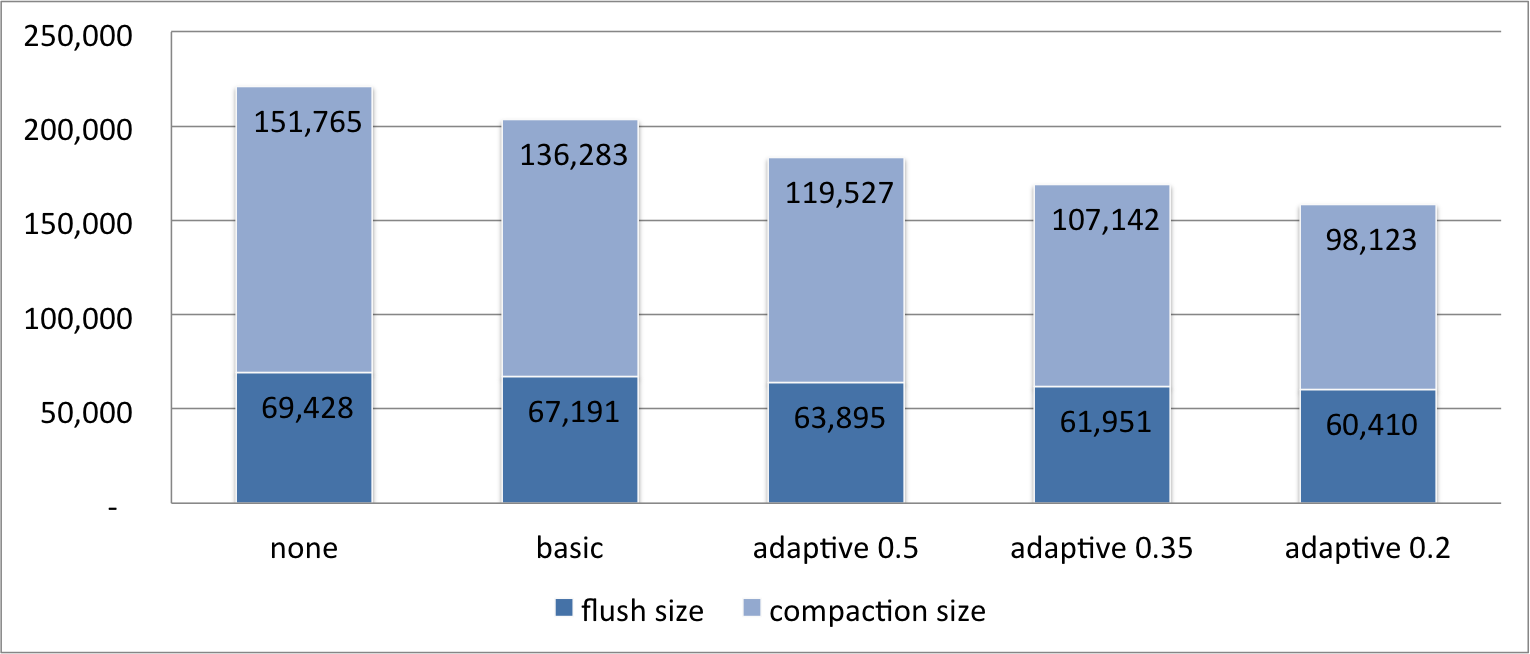
\includegraphics[width=\figw]{Figs/volume-hdd.png}
\caption{{\bf  Write volume in HDD.} Zipfian distribution.
}
\label{fig:volume-hdd}
\end{figure}

Figures~\ref{fig:throughput-ssd-uniform} and~\ref{fig:throughput-hdd-uniform} depict the throughput results with uniform distribution in ssd and hdd, respectively.
Tables~\ref{fig:counters-uniform:ssd} and ~\ref{fig:counters-uniform:hdd} present the number of flushes, disk compactions and WAL files generated during the experiment.
Figures~\ref{fig:volume-ssd-uniform} and~\ref{fig:volume-hdd-uniform} depict the write volume in every setting. 


\begin{figure}[htb]
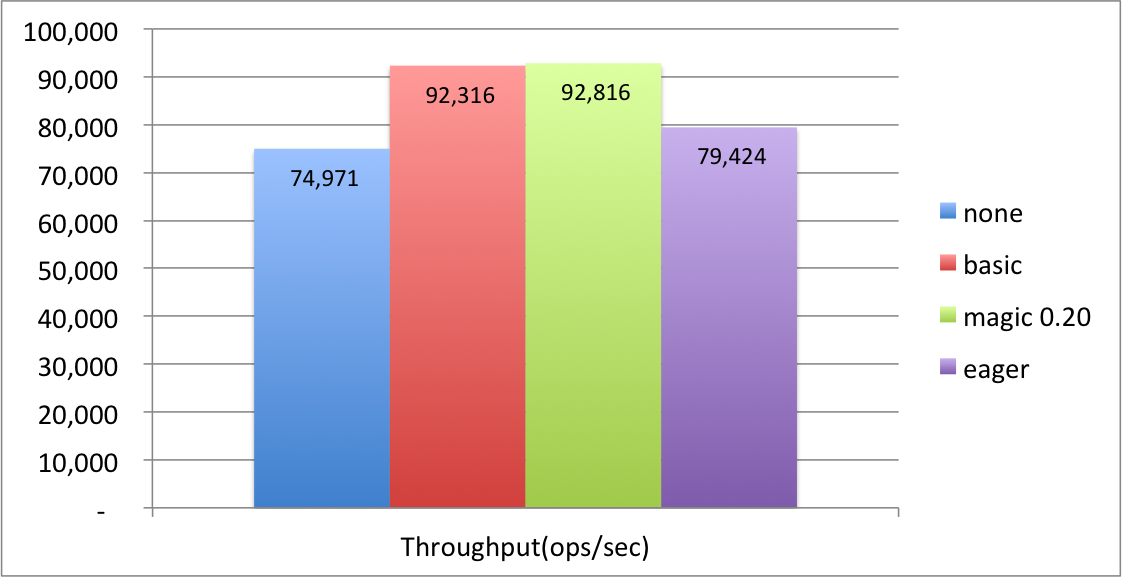
\includegraphics[width=\figw]{Figs/throughput-ssd-uniform.png}
\caption{{\bf  Throughput measured in SSD.} Uniform distribution.
}
\label{fig:throughput-ssd-uniform}
\end{figure}

\begin{figure}[htb]
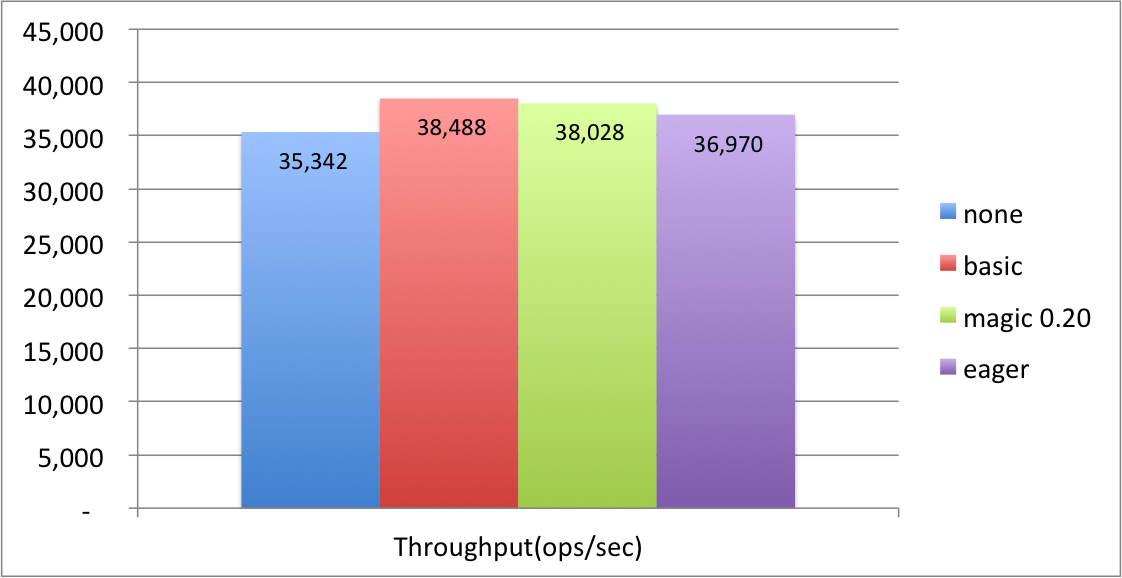
\includegraphics[width=\figw]{Figs/throughput-hdd-uniform.png}
\caption{{\bf  Throughput measured in HDD.} Uniform distribution. 
}
\label{fig:throughput-hdd-uniform}
\end{figure}


\begin{figure}[!t]
  \centering
  
  \begin{subfigure}[tb]{\columnwidth}
      \centering\small
    \begin{tabular}{|c|c|c|c|}
      \hline
      Strategy & $\#$flushes & $\#$compactions & $\#$WAL files\\
      %\hline
      \hline
\none & 1705 & 288 & 632 \\
\basic & 1416 & 220 & 577 \\
\magic\ 0.20 & 1402 & 219 & 586 \\
\eager\ & 1382 & 255 & 578 \\
       \hline
    \end{tabular}
	\caption[]{SSD}
    \label{fig:counters-uniform:ssd}
  \end{subfigure}
  
  \begin{subfigure}[t]{\columnwidth}
    \centering\small
    \begin{tabular}{|c|c|c|c|c|}
      \hline
        Strategy & $\#$flushes & $\#$compactions & $\#$WAL files\\
      %\hline
      \hline
     \none & 1736	&570&	739 \\
\basic & 1408&	458&	742 \\
\magic\ 0.20 & 1413	&470	&770 \\
\eager\ & 1423	&476&	760 \\
      \hline
    \end{tabular}
	\caption[]{HDD}
    \label{fig:counters-uniform:hdd}
  \end{subfigure}


  \caption{Number of flushes, disk compactions, and WAL files created in different settings with uniform distribution}
  \label{fig:counters-uniform}
\end{figure}


\begin{figure}[htb]
%\includegraphics[width=\figw]{Figs/volume-ssd-uniform.png}
\caption{{\bf  Write volume in SSD.} Zipfian distribution.
}
\label{fig:volume-ssd-uniform}
\end{figure}

\begin{figure}[htb]
%\includegraphics[width=\figw]{Figs/volume-hdd-uniform.png}
\caption{{\bf  Write volume in HDD.} Zipfian distribution.
}
\label{fig:volume-hdd-uniform}
\end{figure}



\paragraph{Mixed workload.}
Each run is comprised of two phases. 
The first phase creates an empty 50 regions table. It then loads the table with 10GB of data by running 100 million update operations chosen uniformly at random, each writing to all columns. 
The second phase measures the performance of a single thread running 150,000 read operation. 
We measure the 50-th, 75-th, 90-th, 95-th and 99-th percentiles.
An additional YCSB client is used to run background traffic. 
This client utilizes 12 threads to run update operations while we measure the read operations. 
Both reads and background traffic are chosen from a zipfian distribution.
Each such run is repeated 3 times. 

Figure~\ref{fig:latency-speedup-hdd} depicts the latency speed-up \basic\ and \magic\ achieve over \none.

\begin{figure}[htb]
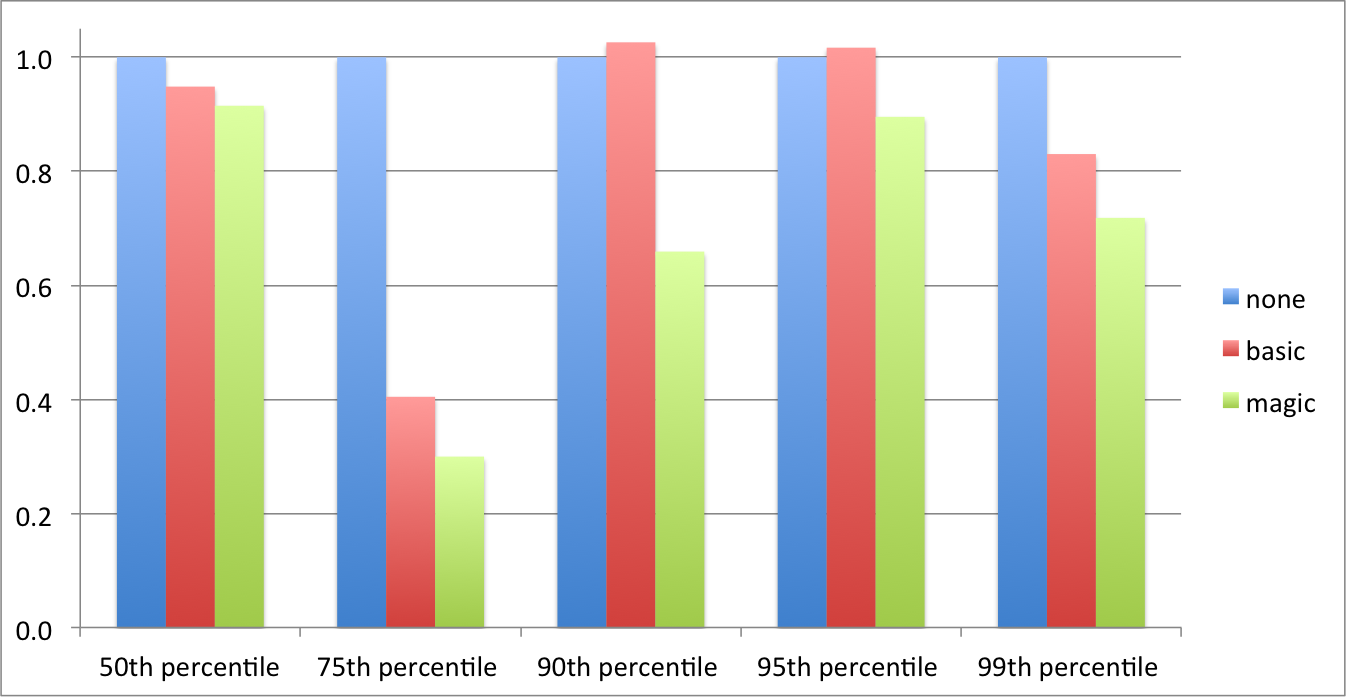
\includegraphics[width=\figw]{Figs/latency-speedup-hdd.png}
\caption{{\bf Latency speed-up in HDD.} 
}
\label{fig:latency-speedup-hdd}
\end{figure}

\paragraph{Parameter exploration.}
One of the main sources for memory management overhead is the skip-list data structure used to index the dynamic fraction of the memory component.
Not only it is bigger in size compared to a flat index it is also fragmented whereas static index is stored in a consecutive block of memory, therefore it incurs smaller overhead in terms of allocation, gc and cache misses.
We evaluate \basic\ strategy with different dynamic fraction sizes. We measure their throughput in write-only workload with zipfian distribution.
The throughput results of all runs are depicted in  Figure~\ref{fig:dynamic-fraction}. 
The \none\ strategy has no static portion in the memory component therefore its throughput is added at the point where the dynamic fraction size is equal to 1.0.
Figure~\ref{fig:dynamic-fraction} shows that indeed the store scales as the dynamic fraction size decreases. 

\begin{figure}[htb]
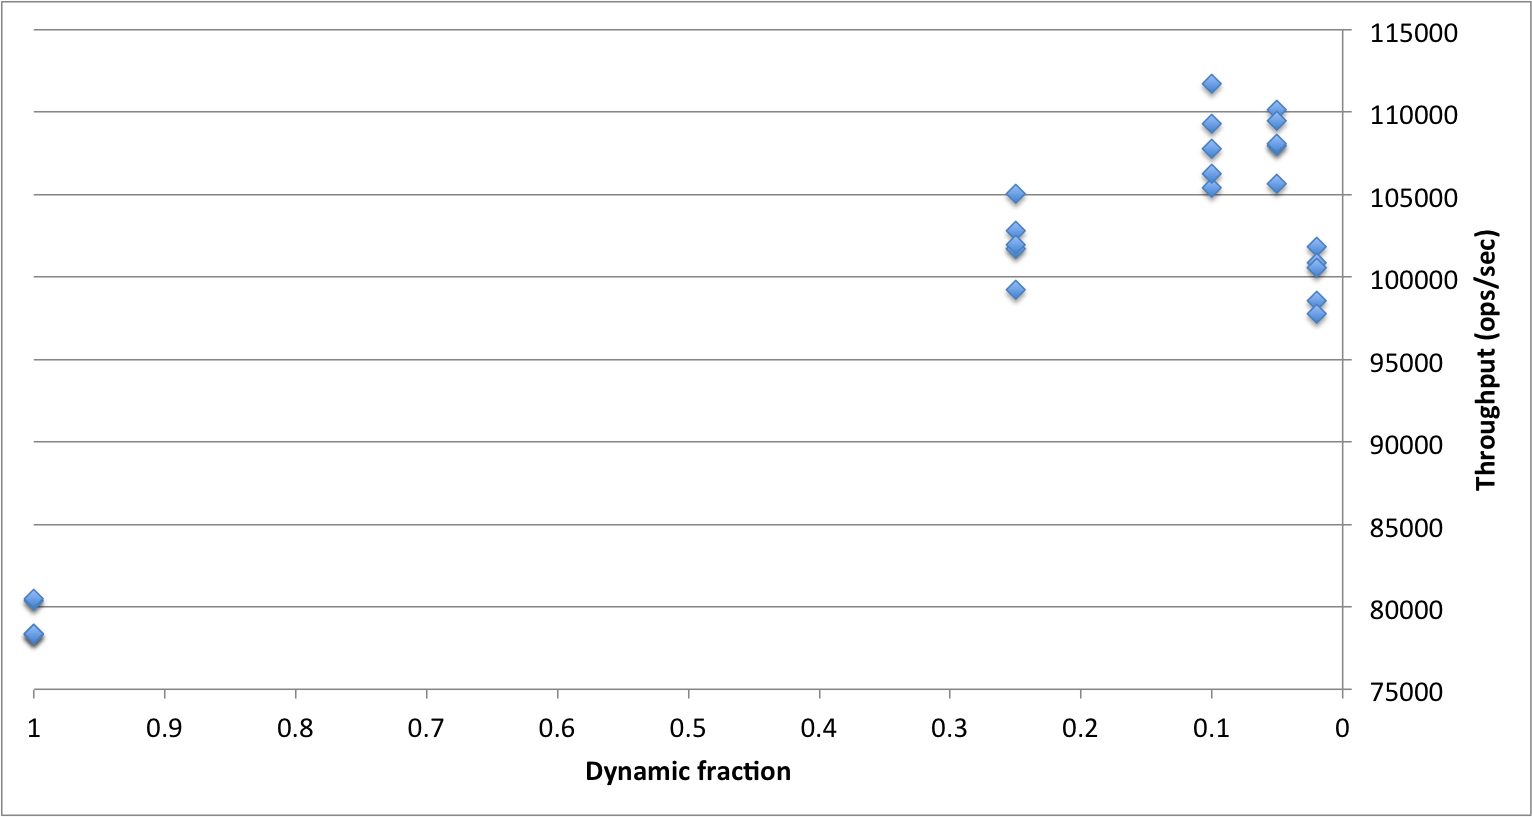
\includegraphics[width=\figw]{Figs/dynamic-fraction-1.png}
\caption{{\bf Dynamic fraction tuning.} The throughput increases as the dynamic fraction size decreases.
}
\label{fig:dynamic-fraction}
\end{figure}

When the dynamic fraction is less than $10\%$ it is clear that merging it into the much bigger static data over and over again can be inefficient as it creates a new index and dismisses the old one. 
The alternative is to enable several segments to wait in the pipeline before they are merged to a single segment. This helps with creating new index less frequently.
On the flip side, each segment in the pipeline calls for a separate scanner during read operations which can degrade their performance.
%Hence, we run the same experiments as explained above, varying the limit for the size of pipeline.
Figures~\ref{fig:pipeline-1-ssd} and~\ref{fig:pipeline-1-hdd} depict the throughput results as a function of the pipeline size. Peak throughput is with XX entries in the pipeline.

\begin{figure}[htb]
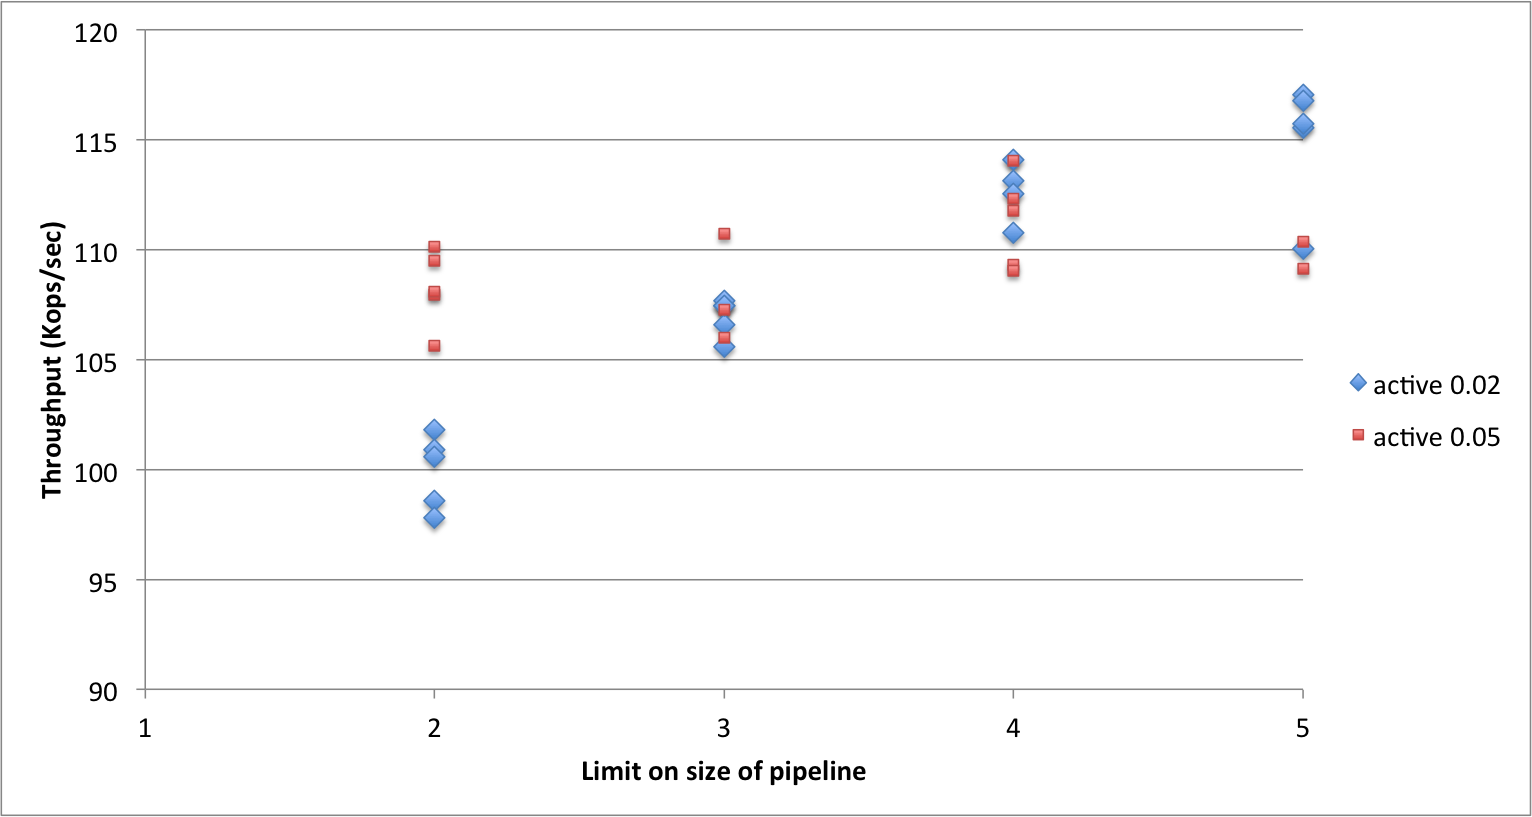
\includegraphics[width=\figw]{Figs/pipeline-1-ssd.png}
\caption{{\bf Pipeline size tuning - SSD.} 
}
\label{fig:pipeline-1-ssd}
\end{figure}

\begin{figure}[htb]
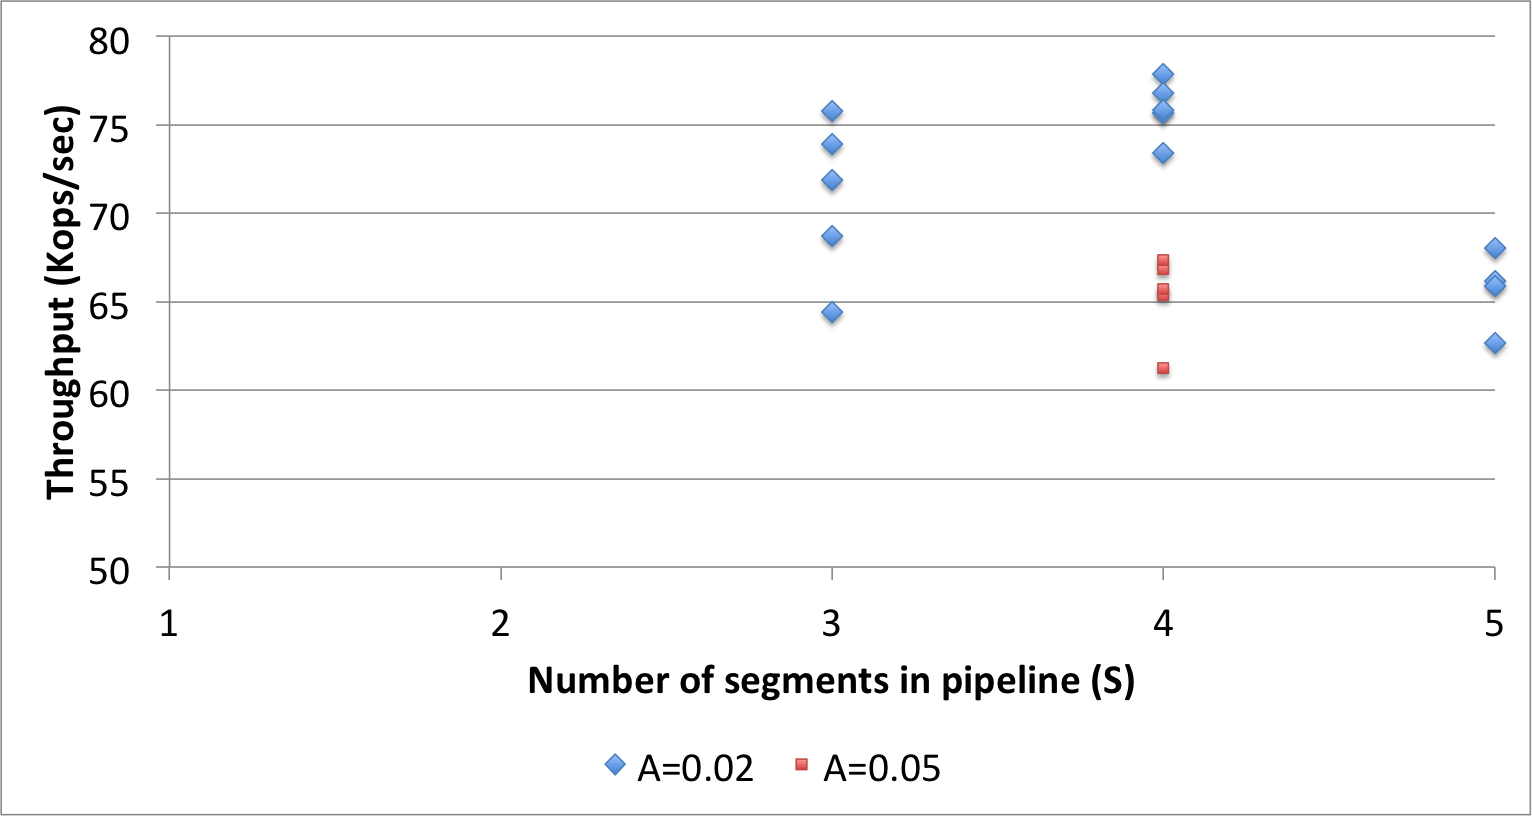
\includegraphics[width=\figw]{Figs/pipeline-1-hdd.png}
\caption{{\bf Pipeline size tuning - HDD.} 
}
\label{fig:pipeline-1-hdd}
\end{figure}

With a different experimental setup the tuning results are different.
For example when running similar workload with 100 regions and 16GB heap per region server we get different results.
\begin{figure}[htb]
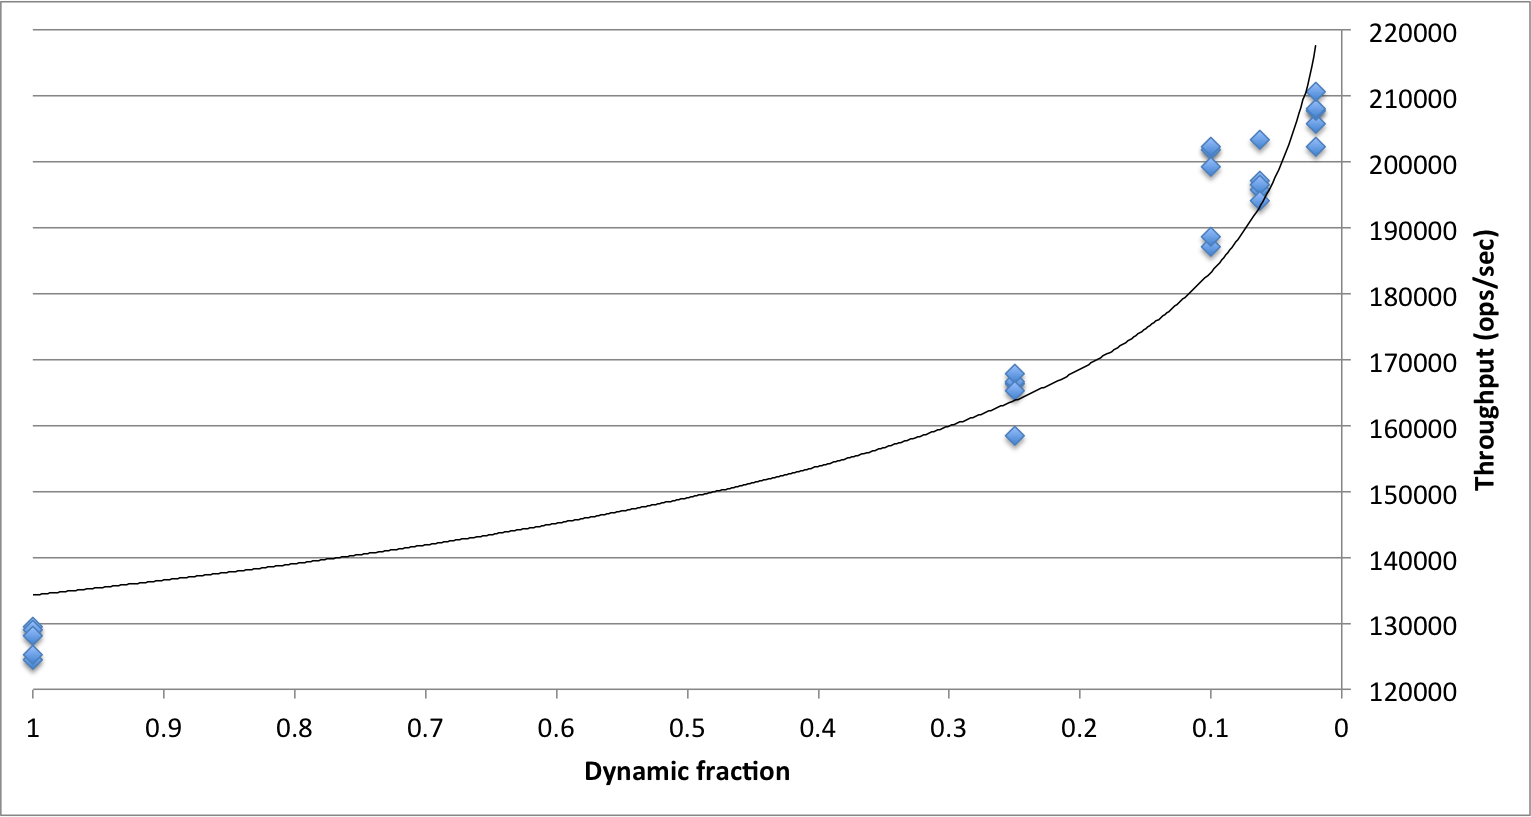
\includegraphics[width=\figw]{Figs/dynamic-fraction-2.png}
\caption{{\bf Dynamic fraction tuning.} 
}
\label{fig:dynamic-fraction-2}
\end{figure}

\begin{figure}[htb]
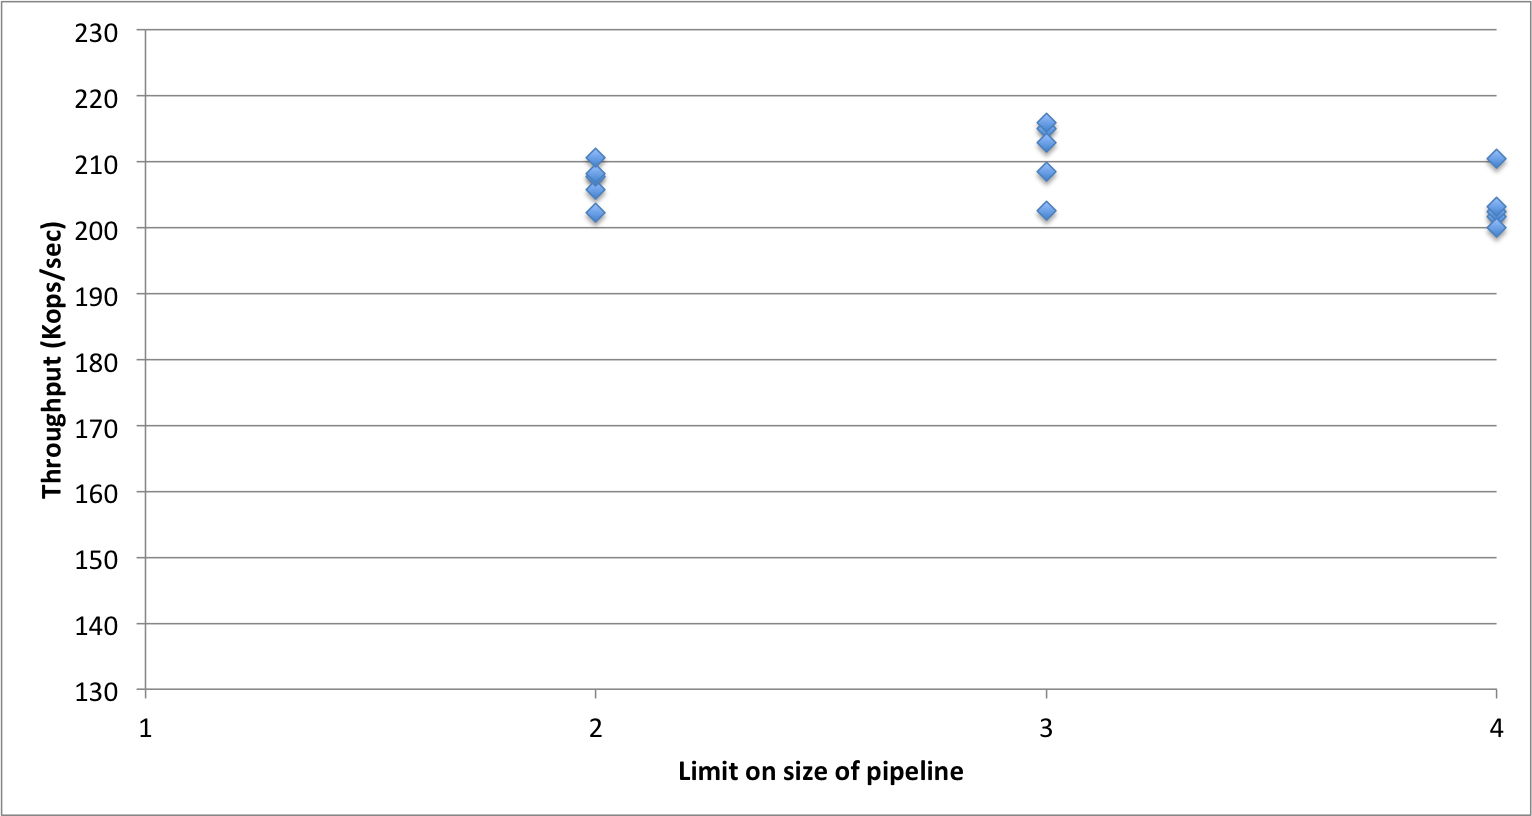
\includegraphics[width=\figw]{Figs/pipeline-2.png}
\caption{{\bf Pipeline size tuning.} 
}
\label{fig:pipeline-2}
\end{figure}

